\chapter{Background}
Before setting off to outline what has been finished in the project and how certain choices were made in comparison to others, the report will be discussing the current situation of the robotics community and the human-robot collaboration in general for how the robots communicate with each other. Also a more detailed outline onto the treasure hunt game will be given to give a better image of why this research was chosen over others.

    With this in mind, it is important to outline what ideas are currently looked at and how they influence the field of robotics and more importantly, what they bring to the project. In the following sections, an outline of the treasure hunt game along with two main areas of research in robotics that are relevant to this report will be given. These evaluations will be concerning human-robot collaboration and research that was focused around the ROS environment.

    \section{Treasure Hunt Game}
      Following the introduction that said that this report will focus on creating a treasure hunt game, it is important to understand the concepts behind the game. The games aim is not to create a competitive game where users will interact. The main goal is to test the communication between various robots. With that said the following explanation will give an outline to how the game works and this explanation is directly inspired by Sklar and Azhar’s paper on ArgumentationBased Dialogue Games for Shared Control in Human-Robot Systems.

      The game works by using a simulation environment between a robot and a human. In this environment there is a map with hidden treasures, a robot that explores it as well as a human suggesting where the robot should go. The person that controls the robot gives commands as to which room the robot should visit first along with an option to ask the robot for its opinion on the matter. This gives room to possibilities of dialogue communication between two parties and as such give a robot the chance to persuade the user towards a better option.

      There are numerous possibilities for the treasures and their identification is important to yield different results as well as to use as little energy as possible to get a maximum score. This score can then be evaluated to see how the robot influenced the user and how the communication influenced the experience for the human as well as the score. This then can be used to decide the best strategy for dialogues. The possibilities for treasures can be demonstrated by a figure taken from Sklar and Azhar’s paper[1] which can be found below for ease of access.

        \begin{figure}[!ht]
          
          \centering
            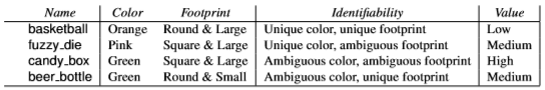
\includegraphics[width=1.02\textwidth]{figures/treasures.png}
            \caption{Example of Treasures in the game.}
        \end{figure}

      With these treasures it is easy to see how users might make errors between treasures that carry high ambiguity but also shows how it is unnecessary to use up energy for taking pictures of treasures that have very unique qualities and with that, can be simply grabbed for increasing the score. This could be developed in the environment to ensure that the robot makes sure that the user is certain of taking pictures of treasures that are implicitly unique.

      The game also makes the robot energy a precious resource with robot losing energy for practically every action that it takes apart from communicating with the user.

      This leads to the motivation in this report of creating this environment with customizability of Dialogues as well as ensuring that a multi robot environment is allowed to further see how increasing the number of robots affect the dialogue experience in Human-Robot communication.

    \section{Related work in Human-Robot collaboration}
      Currently research is greatly focused on human-robot collaboration for humans and robots in the same environment, working simultaneously on a task together. This in turn makes the current problem more unique. The problem we consider in this paper works on the assumption that humans and robots are in separate environments, and with that the robot can potentially have a lot of control over the environment. The following subsections give a more precise background in research of human-robot collaboration.

      \subsubsection{Same space collaboration}
        In their papers Liu et al.\cite{ChangLiu} and Govindarajan et al.\cite{Vijay} discuss collaboration in same space. 

        In the first paper\cite{ChangLiu} the collaboration is outlined by robot working together with the human. The setup of the experiment was to give each human-robot team a group of tasks that either required one agent to complete or a joint task for both of them. The aim was to finish a list of tasks as quickly as possible. The measurement parameters were mainly the fluency of collaboration outlined by Hoffman's metrics. Their results found many conclusions; one of which was that humans preferred working with robots that could infer plans based on human movement. This gives an implication to the project that ultimately guides the project to try and develop a robot that could propose movements as to giving the human full power over the environment and the process. In that way it can be considered good practice to let an idle robot move based on its own path planner to the closest room if it was neglected. This of course, is subject to human preference but allowing such functionality could be considered.

        In Govindarajan et al's\cite{Vijay} paper the main focus of research was search and rescue actions where robots infer different paths from where the human is headed thus maximizing the search space of a room. To develop an algorithm that would handle the robots, the researchers used the ROS platform. In their results they have found that using complementary homotopy classes for intelligent path finding increased the performance of robots helping them make more intelligent decisions. While not particularly useful for robots that search different rooms, using homotopy classes for finding out which robot should potentially reach specific rooms could be useful when making plans that revolve around finding maximum number of rooms helping robots achieve more efficient paths. Additionally another area of research would be with large amount of robots. In that research the robots would use homotopy classes to make decisions based on first movements of robots to try and predict which would be the next rooms that the current robot would choose. With that, the robots would move away from that area that will potentially be visited anyway to start exploring other areas.

      \subsubsection{Spatial recognition}
        Goto et al.'s\cite{Hiraki} paper work on maximizing fluency in human-robot collaboration and identifying challenges posed by robots when it comes to recognizing parts that would be required for assembly of parts. To achieve this they focused on a finite state machine approach for robots to help with table assembly. This can be considered a more limited approach in terms of robot intelligence since robots are limited in the amount of states they will be in. In their results they managed to see limitations with the robot both recognizing the human action and with the scalability of the software due to most of it being hand made beforehand. The paper mainly focused on being able to achieve the task in comparison to achieving the task efficiently or effectively. With that in mind it poses considerations that need to be taken when looking at robot design one of the most important being a challenge being the robot understanding what it sees and how limited they can be when it comes to object recognition.

      \subsubsection{Modalities of human preference}
        While in their paper Fiore et al.\cite{Fiore} did not use the robot operating system, they embarked on a task that would prove that robots are capable of completing collaborative tasks based on human supervision. In this sense, their paper is very related to research outlined in this paper. Fiore et al. Propose a complex system that is built on sophisticated software for intention inference, path planning, task execution and communication. In their results they have proved that the system is capable of: handling joint goals and actions, handling users preferences, handling agent beliefs and monitoring human actions. With that in mind, a multitude of research has been proposed in creating human-robot collaboration and proving that the tasks are in fact possible complete.

      \subsubsection{Conclusion}
        It seems that a lot of current research has put a great focus on proving that human robot collaboration is indeed possible with a huge variation of approaches between each paper. While quite a new area, it is important to note that currently, there doesn't seem to be a greater standard in how research is carried out with researchers assembling software based on their research preference. It does not dispute the fact that every research paper proposes new considerations in human-robot collaboration and that possible improvements are drawn based on their approaches.

        This leads to a conclusion that Human-Robot collaboration is a very undeveloped field and will start presenting more exciting opportunities in the future for researchers to look at. Currently it seems that a great deal of effort is in ensuring that fluency between agents is maximized making the experience faster and more enjoyable for the participant in the study and potential agents for developed systems in the future.
    
    \section{Research in ROS environment}
        The reason for choosing to research ROS in greater detail is that it will be the main platform that runs the robotics simulations in this Project. In essence, it will be the backbone of the system and a lot of work will be determined by the success of its implementation. To achieve this, a solid background on how it was used in the past and what it has been used for is considered to ensure that the wheel has not been reinvented as well as to see potential uses of ROS to later on expand the system when it is developed.

        In comparison to previous research that focused on proving various possibilities of robotics systems, research that focuses on using ROS environment is mostly aimed towards developing various frameworks to ease the use of the environment to achieve certain results. As such, it can be compared to human-robot collaboration research as focusing more on solving problems than proving. Following sections outline various works that used the ROS environment to achieve their goals.

      \subsubsection{Frameworks}
        In their two papers Fok et al.\cite{ChienLiang} and Liang S Ng et al.\cite{Liang} focus on creating two separate networks that provide an interface for grabbing robots and control for complex whole body robots with multiple parts. In both of the papers, ROS was being used which stands to justify just how powerful ROS can be in manipulating various environments. In fact, the paper on creating a hardware and software problem for intelligent applications, is very similar to the approach this report is focused on. The simulation platform is in fact exact with the only difference being controlling single robots forwards and backwards rather than using path planning for the problem. From these findings, given time, the report can be further studied to include complex body robots that can be controlled over the cloud with hand held devices. This only signifies the availability of technology for implementing complex robot systems using ROS.

      \subsubsection{Domain specific research}
        Deusdado et al.'s\cite{Pedro} research focused on creating an aerial-ground teams in ROS for systematic soil and biota in estaurine sampling. Mario Vieira et al.'s research further focused on creating applications for monitoring human daily activity and risk situations in robot-assisted living. Both of these papers can be considered extremely centered around the areas that they focus on and show the variety of scenarios that ROS can be used for. Both teams achieved great success in their plan to centralize use of ROS for their respective goals and showed how useful they can be in further research. The first paper gives us an idea of how ROS can be used to implement robot teams, giving us ideas about how to space out cloud platforms to further enrich the environment while the second, allows us to see how to use robot sensors to view activity of humans. 

        This knowledge, can in fact be extrapolated to the project in future works to give a richer environment. One where each robot is directly responsive to actions of the other through the use of sensors rather than shared goal reaching creating a more human like collaboration not only between the robot and the human but throughout the whole team. It is important to note that while right now the robots focus is to reach desired destinations and share data to produce better maps. An alternative of proposed research above shows us that using a more intuitive approach can be just as useful.

      \subsubsection{Conclusion on ROS research}
        It is very easy to see that ROS research and implementations revolves around creating better frameworks and centralized domain problem solving. It is a very young field that so far didn't set standards towards what would be the best approach so that researchers could start tackling these issues and start improving on standard solutions. This in turn, emphasizes that the field is going to expand creating more elaborate solutions and frameworks for specific domain problems. At the time this report was written, most papers presented here are papers that came out in 2016th to ensure that the image of current affairs is as accurate as possible. With this information, as presented above ideas can be drawn about possible improvements to the implementation that could in turn create an environment where the collaboration is as fluent as possible with robots taking same type of initiative that normal humans would.

      \section{ROS challenges posed by its creators and community}
        Currently ROS is an overwhelmingly expanding software with new additions being added. ROS started in 2010 and already had 9 releases with the 10th coming out in May 2016. This sort of expansion rate pushes developers to re-learn the structure and standards set by ROS every few months, in turn making the frameworks obsolete every 8 months or so IF they used code that ROS creators deemed unnecessary in future releases or made it deprecated through certain decisions. This challenge is actually an obstacle for ROS creators themselves as in some examples, the Wiki pages can reference functions that can be considered deprecated in future releases. This in turn makes developers turn to the ROS community which is limited to the small group of robotics specialists using ROS that are willing to help on answers.ros.org.

        The community itself is compromised of a fairly small amount of user group that cannot be compared to regular software developer websites like StackOverflow or BigResource where commercial development and advice seeking can start to compare itself to a competition of its own. This produces problems when a regular developer that didn't have much experience with the environment, thus making it harder to develop in this network.

        It is also extremely important to note that at this point in time there is a huge deficit in the amount of available resources the developer can reference to when it comes their struggles. The few books that do exist to help users develop their knowledge are few and their knowledge as previously stated can become obsolete extremely fast due to ROS's quick expansion rate. When this report was created, there were also no current frameworks available for faster safer development or third party libraries to help a developer create a bigger understanding which means that the wheel of development for ROS is mostly reinvented every time a new idea is presented for development. This leads to a conclusion that the outlined specification will be extremely challenging posing a lot of stalls for implementation of the software.
        
    \section{Conclusion}
      It is clear that ROS is an amazing platform offering its users a great diversity in use. The research in human-robot collaboration and ROS is starting to expand the use of ROS in human-robot collaboration is starting to slowly become a standard. This in turn means, that selecting ROS as a developer platform for robot simulation is definitely a right fit for this project.

      With the previous section, it is clear that there will be challenges in this project that might in fact not get fulfilled simply due to lack of resources that will be able to acquire and through that, a careful consideration will be taken to ensure that the goals are realistic and not reaching outside the scope of the possibilities.